\begin{titre}[Les statistiques]

{\color{bleu3}{\LARGE Lecture et représentation de données} \hfill{Niveau 2}}
\end{titre}



\begin{CpsCol}
\textbf{Interpréter, représenter et traiter des données}
\begin{description}
\item[$\square$] Lire des données sur différents supports
\end{description}
\end{CpsCol}

\begin{AD}

Les notes d'une classe de Seconde sont représentées par le diagramme à bâtons ci-dessous.

\begin{center}
\definecolor{ffqqqq}{rgb}{1.,0.,0.}
\definecolor{cqcqcq}{rgb}{0.7529411764705882,0.7529411764705882,0.7529411764705882}
\begin{tikzpicture}[line cap=round,line join=round,>=triangle 45,x=1.0cm,y=1.0cm]
\draw [color=cqcqcq,, xstep=1.0cm,ystep=1.0cm] (-0.76,-1.1175) grid (11.64,7.2625);
\draw[->,color=black] (-0.76,0.) -- (11.64,0.);
\foreach \x in {,1.,2.,3.,4.,5.,6.,7.,8.,9.,10.,11.}
\draw[shift={(\x,0)},color=black] (0pt,2pt) -- (0pt,-2pt) node[below] {\footnotesize $\x$};
\draw[->,color=black] (0.,-1.1175) -- (0.,7.2625);
\foreach \y in {-1.,1.,2.,3.,4.,5.,6.,7.}
\draw[shift={(0,\y)},color=black] (2pt,0pt) -- (-2pt,0pt) node[left] {\footnotesize $\y$};
\draw[color=black] (0pt,-10pt) node[right] {\footnotesize $0$};
\clip(-0.76,-1.1175) rectangle (11.64,7.2625);
\draw [line width=2.pt,color=ffqqqq] (1.,0.)-- (1.,2.);
\draw [line width=1.2pt,color=ffqqqq] (2.,0.)-- (2.,3.);
\draw [line width=1.2pt,color=ffqqqq] (3.,0.)-- (3.,2.);
\draw [line width=1.2pt,color=ffqqqq] (4.,0.)-- (4.,4.);
\draw [line width=1.2pt,color=ffqqqq] (5.,0.)-- (5.,6.);
\draw [line width=1.2pt,color=ffqqqq] (6.,0.)-- (6.,5.);
\draw [line width=1.2pt,color=ffqqqq] (7.,0.)-- (7.,5.);
\draw [line width=1.2pt,color=ffqqqq] (8.,0.)-- (8.,4.);
\draw [line width=1.2pt,color=ffqqqq] (9.,0.)-- (9.,2.);
\draw [line width=1.2pt,color=ffqqqq] (10.,0.)-- (10.,1.);
\draw (10.08,-0.4975) node[anchor=north west] {note sur 10};
\draw (0.12,6.5425) node[anchor=north west] {Effectif};
\end{tikzpicture}
\end{center}

\begin{enumerate}
\item Quelle est la note plus plus souvent obtenue ? Cette valeur s'appelle \textbf{le mode}.
\item Combien d'élèves composent cette classe ?
\end{enumerate}

\end{AD}

\begin{AD}

Évolution de la population chinoise

\begin{center}
\begin{tabular}{|c|c|c|}
\hline 
\rowcolor{bleu1!25!white} & 1950 & 2009  \\ 
\hline 
\cellcolor{bleu1!25!white}  Nombre d'habitants &  \np{554760} millions & 1,3 milliards  \\ 
\hline 
\cellcolor{bleu1!25!white} Espérance de vie & 39 & 73 \\ 
\hline 
\cellcolor{bleu1!25!white}IDH ( indicateur de développement humain) & 0,55 (1980) & 0,772 \\ 
\hline 
\cellcolor{bleu1!25!white}Part de personnes sachant lire et écrire (en \%) & H : 79\% et F :54,4\% &  H :94,1\% et F :82,1\%  \\ 
\hline 
\cellcolor{bleu1!25!white}Mortalité infantile (pour 1000 naissances) & 195 & Garçons(17), Filles(24) \\ 
\hline 
\cellcolor{bleu1!25!white}Fécondité & 6,6 & 1,7 \\ 
\hline 
\end{tabular} 
\end{center}

\begin{enumerate}
\item Quelle est l'évolution du nombre d'habitants en Chine entre  1950 et 2009 ?
\item Combien de femmes savent lire en 1950 ? en 2009 ? 
\item Quelle est l'évolution de l'espérance de vie en Chine entre 1950 et 2009 ?
\item Dans un village de \np{1280} habitants comprenant 45\% d'hommes, combien d'habitants savent lire ?
\end{enumerate}


\end{AD}


\begin{AD}

\begin{minipage}{0.5\linewidth}
Le graphique ci-dessous montre les résultats à un contrôle de sciences obtenus par deux groupes d'élèves, désignés par « Groupe A » et « Groupe B ». 
La note moyenne pour le Groupe A est de 62,0 et de 64,5 pour le Groupe B. Les élèves réussissent ce contrôle lorsque leur note est de 50 points ou davantage. Sur la base de ce graphique, le professeur conclut que le Groupe B a mieux réussi ce contrôle que le Groupe A. Les élèves du Groupe A ne sont pas d'accord avec le professeur. Ils essaient de le convaincre que le Groupe B n'a pas nécessairement mieux réussi. \hfill{{\scriptsize D'après PISA 2009}}
\end{minipage}
\begin{minipage}{0.5\linewidth}
\begin{center}
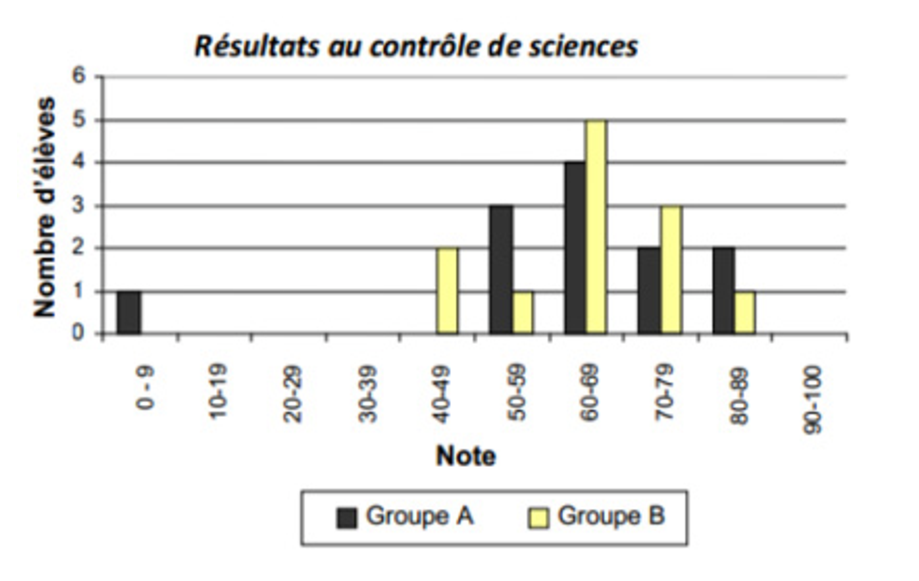
\includegraphics[scale=0.6]{Stat-13.eps} 
\end{center}
\end{minipage}
En vous servant du graphique, donnez un argument mathématique que les élèves du Groupe A pourraient utiliser. 


\end{AD}

\begin{AD}

On a représenté sur le diagramme suivant les vols du mois de février d’une compagnie aérienne.  
\begin{center}
\definecolor{xdxdff}{rgb}{0.49019607843137253,0.49019607843137253,1.}
\definecolor{ffdxqq}{rgb}{1.,0.8431372549019608,0.}
\definecolor{ffffqq}{rgb}{1.,1.,0.}
\definecolor{ffxfqq}{rgb}{1.,0.4980392156862745,0.}
\definecolor{ffqqqq}{rgb}{1.,0.,0.}
\definecolor{xfqqff}{rgb}{0.4980392156862745,0.,1.}
\definecolor{qqqqff}{rgb}{0.,0.,1.}
\begin{tikzpicture}[line cap=round,line join=round,>=triangle 45,x=1.0cm,y=1.0cm]
\clip(-0.096,-0.204) rectangle (18.304,8.336);
\draw[color=xfqqff,fill=xfqqff,fill opacity=1.0] (5.,3.5757359312880714) -- (5.424264068711929,3.5757359312880714) -- (5.424264068711929,4.) -- (5.,4.) -- cycle; 
\draw [shift={(5.,4.)},color=ffqqqq,fill=ffqqqq,fill opacity=1.0] (0,0) -- (0.:0.6) arc (0.:30.488940499830935:0.6) -- cycle;
\draw [shift={(5.,4.)},color=ffxfqq,fill=ffxfqq,fill opacity=0.95] (0,0) -- (30.488940499830935:0.6) arc (30.488940499830935:59.44286434307001:0.6) -- cycle;
\draw [shift={(5.,4.)},fill=black,fill opacity=1.0] (0,0) -- (59.44286434307001:0.6) arc (59.44286434307001:90.:0.6) -- cycle;
\draw [shift={(5.,4.)},color=qqqqff,fill=qqqqff,fill opacity=0.44]  plot[domain=1.5707963267948966:4.71238898038469,variable=\t]({1.*4.*cos(\t r)+0.*4.*sin(\t r)},{0.*4.*cos(\t r)+1.*4.*sin(\t r)});
\draw [shift={(5.,4.)},color=xfqqff,fill=xfqqff,fill opacity=0.66]  (0,0) --  plot[domain=-1.5707963267948966:0.,variable=\t]({1.*4.*cos(\t r)+0.*4.*sin(\t r)},{0.*4.*cos(\t r)+1.*4.*sin(\t r)}) -- cycle ;
\draw [shift={(5.,4.)},color=ffqqqq,fill=ffqqqq,fill opacity=0.6]  (0,0) --  plot[domain=0.:0.5321323971666955,variable=\t]({1.*4.*cos(\t r)+0.*4.*sin(\t r)},{0.*4.*cos(\t r)+1.*4.*sin(\t r)}) -- cycle ;
\draw [shift={(5.,4.)},color=ffxfqq,fill=ffxfqq,fill opacity=0.4]  (0,0) --  plot[domain=0.5321323971666955:1.037473699602908,variable=\t]({1.*3.973415659102379*cos(\t r)+0.*3.973415659102379*sin(\t r)},{0.*3.973415659102379*cos(\t r)+1.*3.973415659102379*sin(\t r)}) -- cycle ;
\draw [shift={(5.,4.)},color=ffffqq,fill=ffffqq,fill opacity=0.5]  (0,0) --  plot[domain=1.037473699602908:1.5707963267948966,variable=\t]({1.*4.*cos(\t r)+0.*4.*sin(\t r)},{0.*4.*cos(\t r)+1.*4.*sin(\t r)}) -- cycle ;
\draw (10.644,6.776) node[anchor=north west] {Vols vers l'Asie};
\draw (10.664,6.176) node[anchor=north west] {Vols vers l'Afrique};
\draw (10.664,5.616) node[anchor=north west] {Vols vers l'Amérique};
\draw (10.704,5.056) node[anchor=north west] {Vols vers l'Europe};
\draw (10.724,4.436) node[anchor=north west] {Vols vers la France};
\begin{scriptsize}
\draw [fill=ffffqq] (10.304,6.636) circle (2.5pt);
\draw [fill=ffdxqq] (10.304,6.036) circle (2.5pt);
\draw [fill=ffqqqq] (10.324,5.436) circle (2.5pt);
\draw [fill=xfqqff] (10.344,4.836) circle (2.5pt);
\draw [fill=xdxdff] (10.364,4.236) circle (2.5pt);
\end{scriptsize}
\end{tikzpicture}
\end{center}

\begin{minipage}{8cm}
Dans chaque cas, quelle fréquence représentent les vols vers la France, l’Europe et l’Asie. 
\end{minipage}
\begin{minipage}{1cm}
$~~$
\end{minipage}
\begin{minipage}{8cm}
Au mois de février, cette compagnie a affrété 576 vols. Calculer le nombre de vols vers la France, l’Europe et l’Asie. 
\end{minipage}

\end{AD}



\begin{autoeval}
\begin{tabular}{p{12cm}p{0.5cm}p{0.5cm}p{0.5cm}p{1cm}}
\textbf{Compétences visées} &  M I & MF & MF  & TBM \vcomp \\ 
Lire des données sur différents supports & $\square$ & $\square$  & $\square$ & $\square$ \vcomp \\ 
\end{tabular}
{\footnotesize MI : maitrise insuffisante ; MF = Maitrise fragile ; MS = Maitrise satisfaisante ; TBM = Très bonne maitrise}
 
\end{autoeval}